%\documentclass[global,referee]{svjour}
\documentclass[]{article}

\usepackage{longtable}
\usepackage{graphicx}
\usepackage{lscape}
\usepackage{multirow}
\usepackage{setspace}


%\chapter{Behavior Tree Language}
%\label{App:BTSyntax}

\begin{document}

\section{Naming Conventions}

\subsection{Variable Naming Conventions}

\begin{itemize}
\item Component names should be capitalised e.g OVEN
\item The first letter of a behavior should be captialised e.g Open
\item The first letter of an attribute should be lowercase e.g. timer
\end{itemize}

\begin{table}[hb]
 \begin{center}
 \begin{small}
 \begin{tabular}{|c|l|}
 \hline
 \textbf{Variable} & \textbf{Description} \\ 
 \hline
 \hline
 $N,N_i$ & Behavior Tree Nodes \\ 
 \hline
 $T,T_i$ & Behavior Trees \\ 
 \hline
 $C,C_i$ & Components \\ 
 \hline
 $C\#$ & A Component Instance \\ 
 \hline
 $s$ & A State of a Component \\ 
 \hline
 $e$ & An Event \\ 
 \hline
 $a$ & An Attribute of a Component \\ 
 \hline
 $b$ & A Branching Condition of a Component \\ 
 \hline
 \end{tabular}
 \end{small}
 \end{center}
 \caption{Variable Naming Conventions}
 \label{Variable Naming Conventions}
\end{table}

\clearpage

\subsection{Node Naming Conventions}

\begin{table}[hb]
\begin{center}
\begin{small}
\begin{tabular}{|c|l|p{0.65\textwidth}|}
 \hline
 \textbf{Label} & \textbf{Name} & \textbf{Description} \\ 
 \hline
 \hline
 A & Component Name & Specifies a component \\ 
 \hline
 B & Behavior & Specifies the behavior associated with the component \\ 
 \hline
 \multirow{2}{*}{C} & \multirow{2}{*}{Operator} & Describes threaded behavior that is linked to the matching node in the tree \\ 
 \hline
 \multirow{2}{*}{D} & \multirow{2}{*}{Label} & An optional label for disambiguation (in case a node appears elsewhere with the same component and behavior)\\ 
 \hline
 \multirow{2}{*}{E} & \multirow{2}{*}{Behavior Type} & Delimiters on the behavior indicating the type of behavior involved \\ 
 \hline
 F & Traceability Link & A reference to the requirements document\\ 
 \hline
 G & Traceability Status & Indicates how the node relates to the traceability link \\ 
 \hline
 \multirow{2}{*}{H} & \multirow{2}{*}{Tag} & The box on the left-hand side of the node (may be omitted in different contexts)\\ \hline
 I & Behavior Tree Node & A node consisting of all or some of the information above \\ 
 \hline
\end{tabular}
\end{small}
\end{center}
\caption{Elements of a Behavior Tree Node}
\label{tbl:BTNodeElements}
\end{table}

\begin{figure}[hb]
 \centering
 \framebox{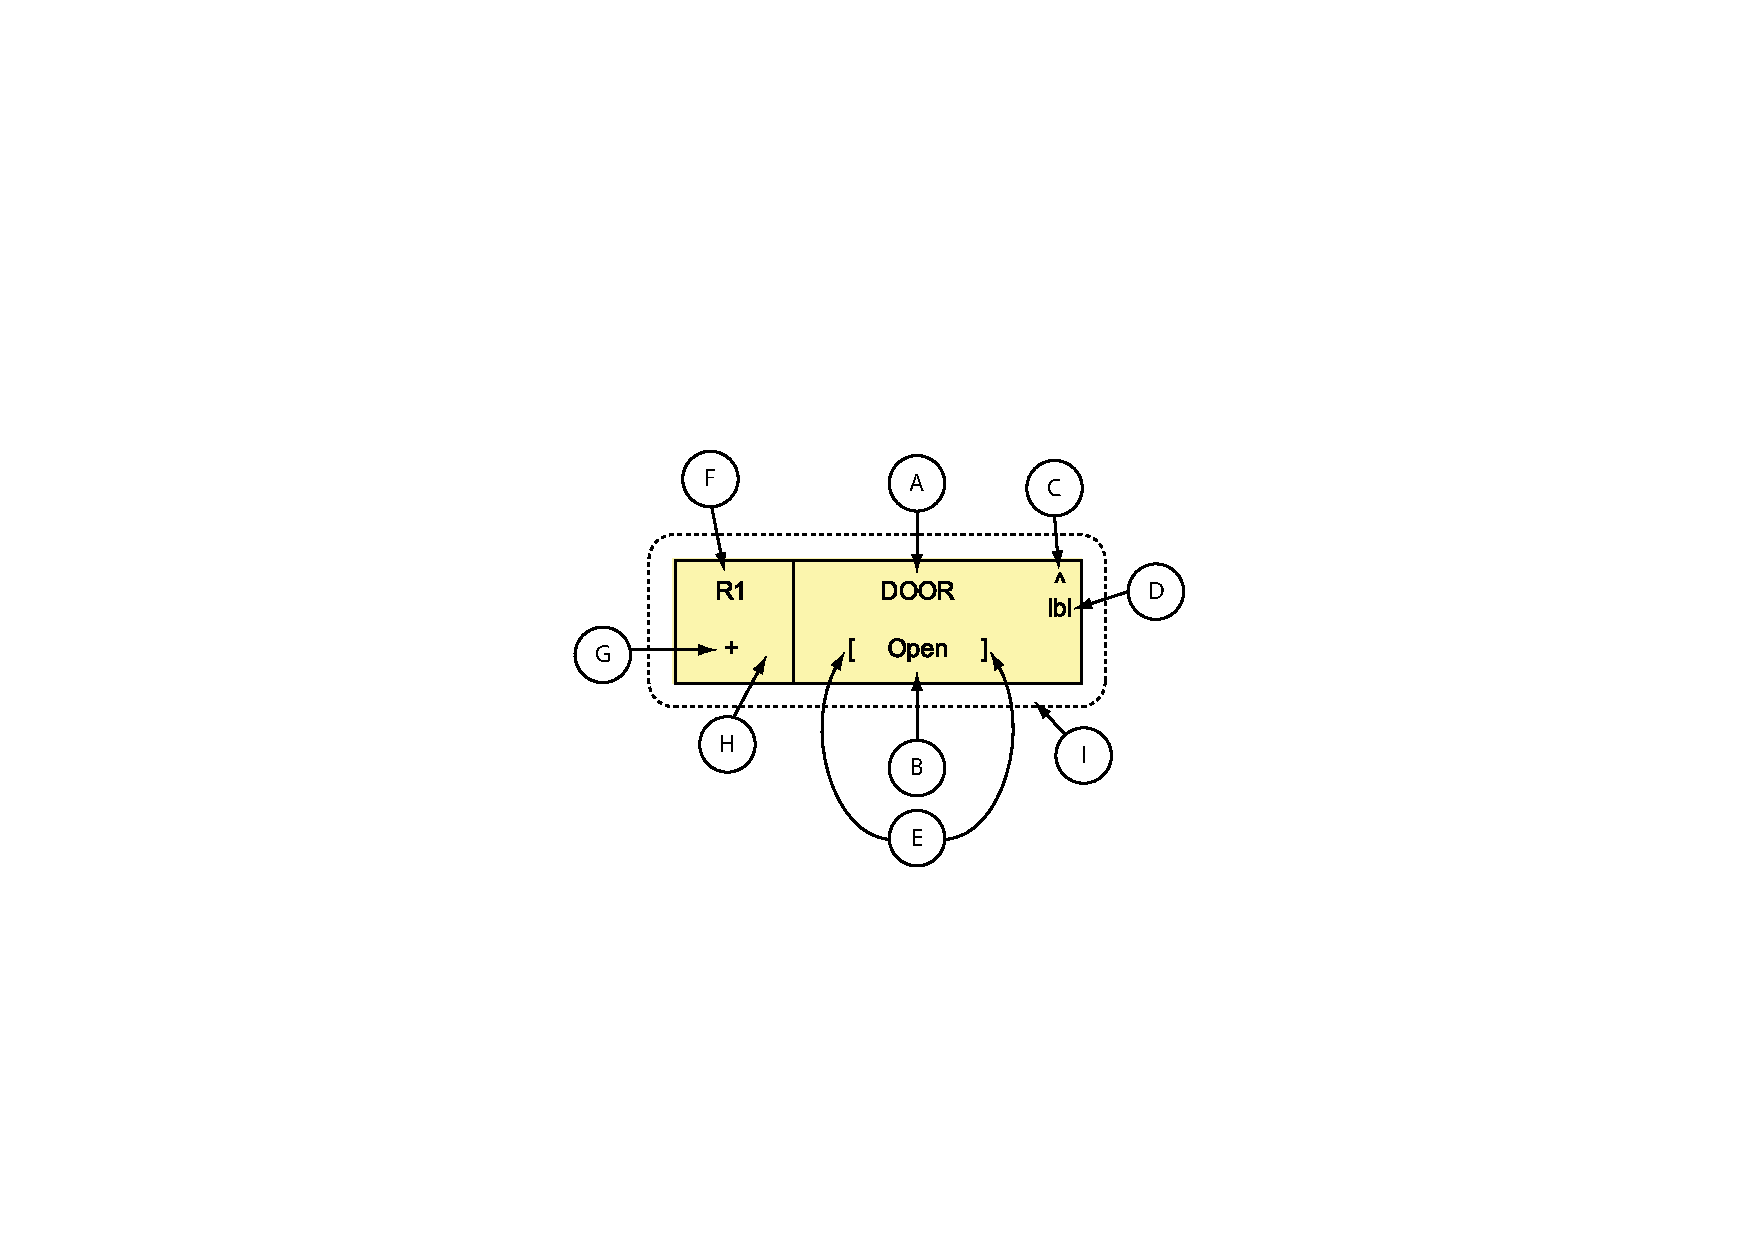
\includegraphics[width=0.6\textwidth]{figs/AppendixB/Naming/Fig1.pdf}}
 \caption{Behavior Tree Node Naming Conventions}
 \label{fig:Naming1}
\end{figure}

\clearpage

\subsection{Relation Naming Conventions}

\begin{table}[hb]
\begin{center}
\begin{small}
\begin{tabular}{|c|l|p{0.65\textwidth}|}
 \hline
 \textbf{Label} & \textbf{Name} & \textbf{Description} \\ 
 \hline
 \hline
 \multirow{2}{*}{A} & Primary Component & \multirow{2}{*}{The component and behavior that form the relation} \\ 
  & \& Behavior & \\
 \hline
 \multirow{2}{*}{B} & \multirow{2}{*}{Related Component} & Component (and optional behavior) related to the primary component and behavior \\ 
 \hline
 \multirow{2}{*}{C} & \multirow{2}{*}{Qualifier} & Specifies the type of the relation. Must be one of What, Where, When, Why, Who or How \\
 \hline
 D & Preposition & Further qualifies the relation to remove potential ambiguity \\
 \hline
 \multirow{3}{*}{E} & \multirow{3}{*}{Secondary Relation} & The related component is linked to the primary component using a forward slash (/). Multi-level relations can be formed by using multiple forward slashes\\
 \hline
\end{tabular}
\end{small}
\end{center}
\caption{Elements of a Behavior Tree Relation}
\label{tbl:RelationElements}
\end{table}

\begin{figure}[hb]
 \centering
 \framebox{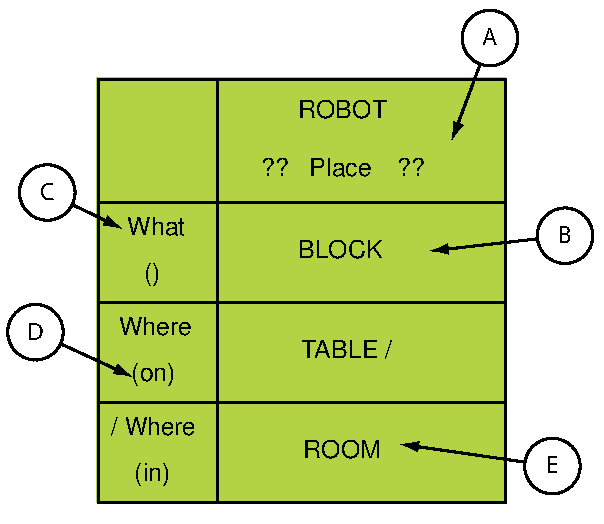
\includegraphics[width=0.5\textwidth]{figs/AppendixB/Naming/Relation.pdf}}
 \caption{Behavior Tree Relation Naming Conventions}
 \label{fig:RelationNaming}
\end{figure}

\clearpage

\subsection{Tree Naming Conventions}

\begin{table}[hb]
\begin{center}
\begin{tabular}{|c|l|p{0.65\textwidth}|}
\hline
 \textbf{Label} & \textbf{Name} & \textbf{Description} \\ 
 \hline
 \hline
 A & Ancestor Node & Any node which appears in a direct line between the node of interest and the root node of the tree\\ 
 \hline
 B & Parent Node & An immediate ancestor\\ 
 \hline
 C & Sibling Node & A node which shares the same parent\\ 
 \hline
 D & Sibling Branch & A subtree with a sibling node as its root\\
  \hline
 E & Child Node & A node immediately below the node of interest\\ 
 \hline
 F & Descendant & Any node appearing below the node of interest\\ 
 \hline
\end{tabular}
\end{center}
\caption{Nodes of a Behavior Tree}
\label{BTTree Nodes}
\end{table}

\begin{figure}[hb]
 \centering
 \framebox{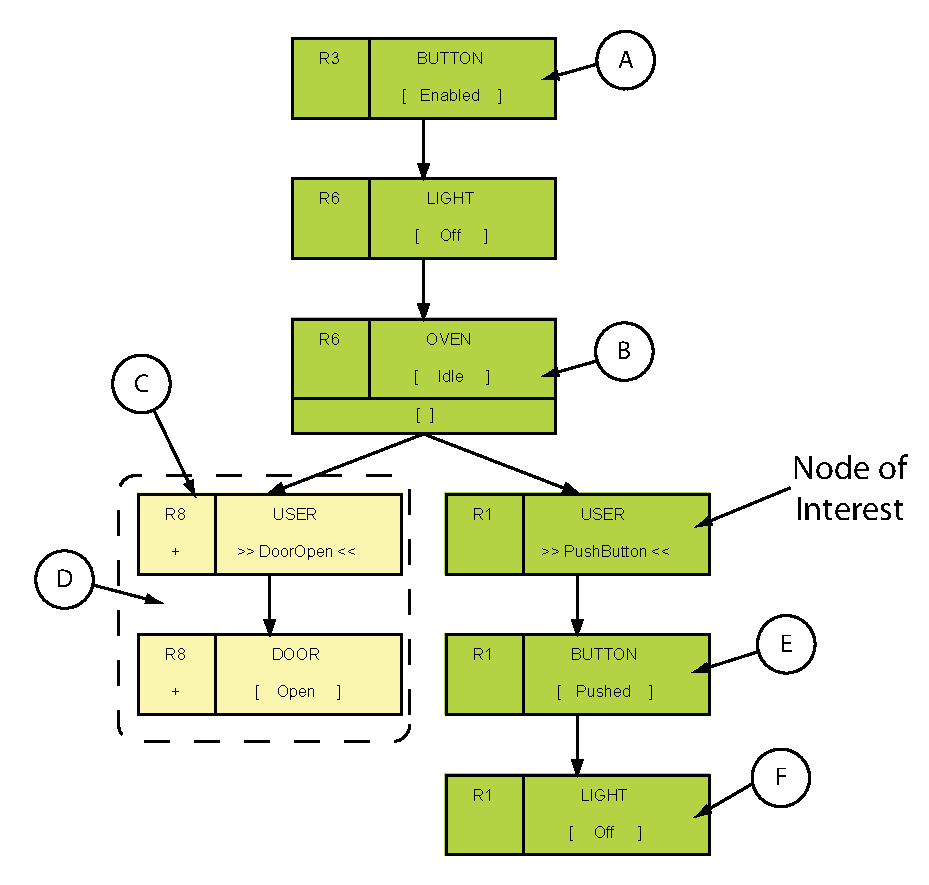
\includegraphics[width=0.75\textwidth]{figs/AppendixB/Naming/Fig2.pdf}}
 \caption{Behavior Tree Tree Naming Conventions}
 \label{fig:Naming2}
\end{figure}

\clearpage

\subsection{Tree Branch Naming Convention}

\begin{table}[hb]
\begin{center}
\begin{tabular}{|c|l|p{0.65\textwidth}|}\hline
 \textbf{Label} & \textbf{Name} & \textbf{Description} \\ 
 \hline
 \hline
 A & Root Node & The first node in a tree (does not have a parent)\\ \hline
 B & Edge & A connection between two nodes \\ \hline
 C & Leaf Node & A node with no children \\ \hline
 D & Branch & A subtree of the node of interest \\ \hline
\end{tabular}
\end{center}
\caption{Branches of a Behavior Tree}
\label{BTTree Branches}
\end{table}

\begin{figure}[hb]
 \centering
 \framebox{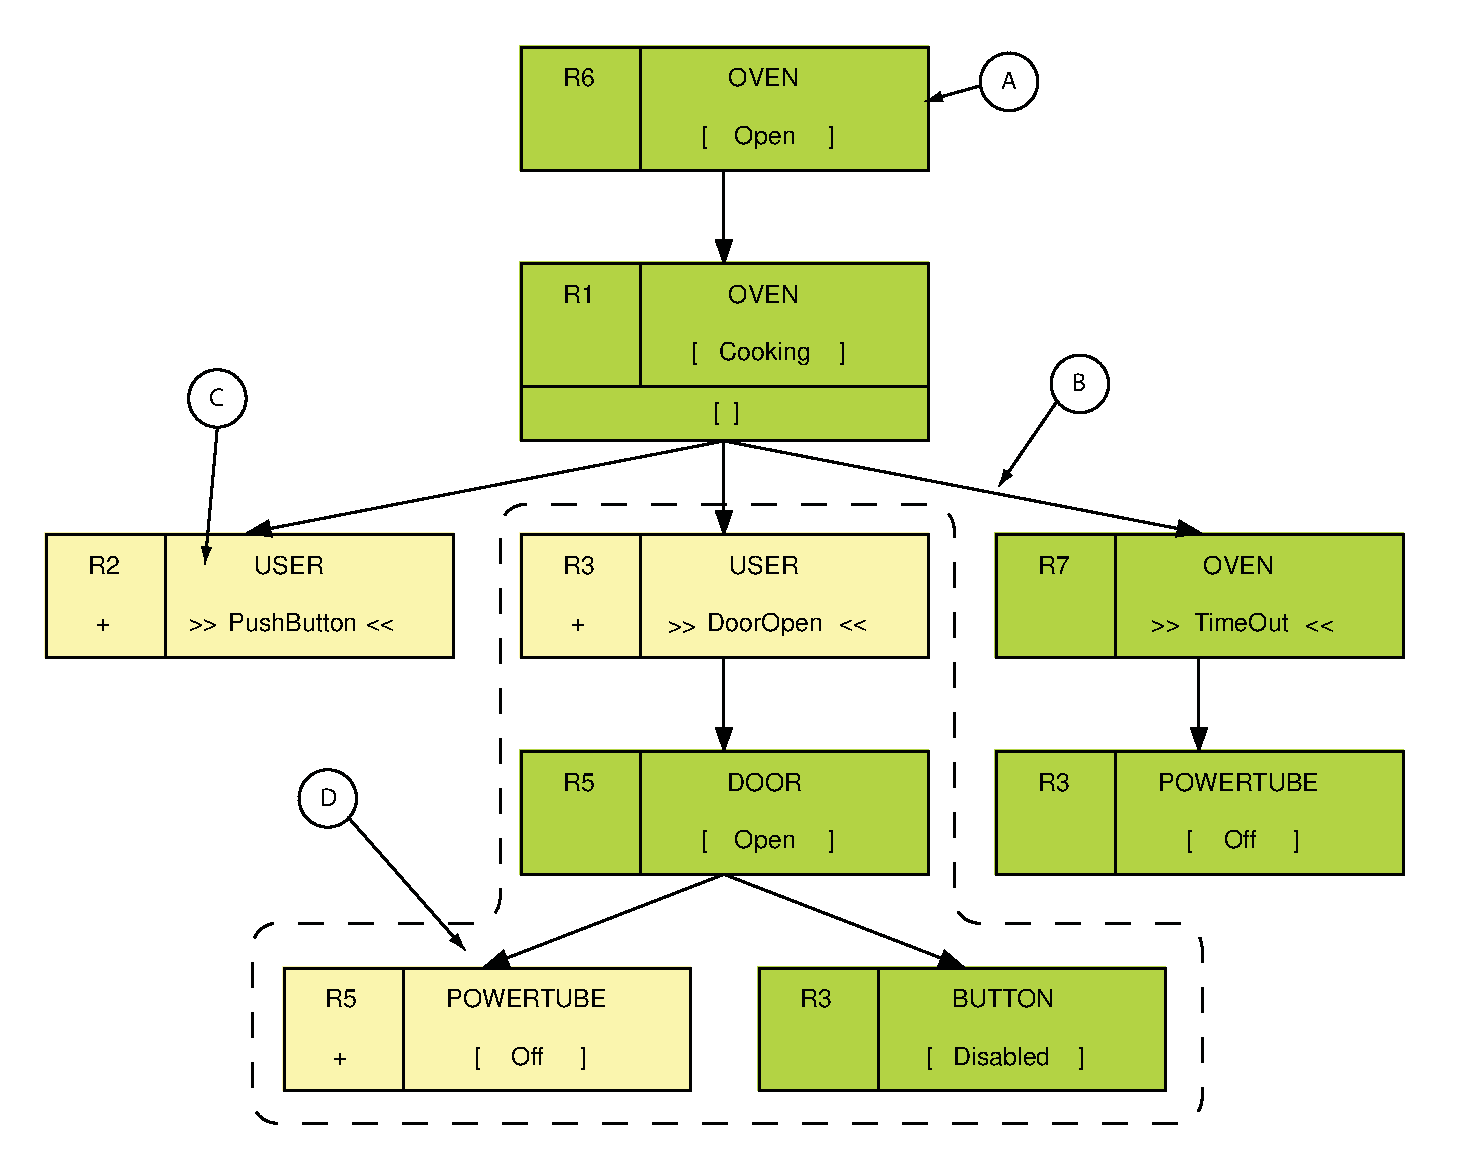
\includegraphics[width=0.85\textwidth]{figs/AppendixB/Naming/Fig3.pdf}}
 \caption{Tree Branch Naming Convention}
 \label{fig:Naming3}
\end{figure}

\begin{landscape}
\section{Behavior Tree Notation \& Syntax}

\subsection{Node Tags}

\singlespacing
\begin{center}
\begin{longtable}[c]{|c|c|p{12cm}|}
\hline
\textbf{Type} & \textbf{Graphical Notation} & \textbf{Description} \\
\hline
\hline
 \multirow{3}{*}{Original} & \multirow{3}{*}{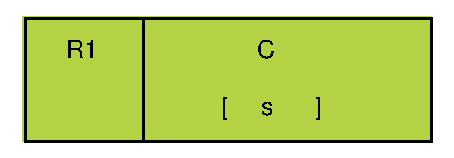
\includegraphics[width=0.23\textwidth]{figs/AppendixB/Tags/Original.pdf}} & \multirow{3}{12cm}{No traceability status indicates that the behavior is stated in the original requirements. The color ``green'' is used for original requirements.} \\*
 &&\\
 &&\\
 \hline
 \multirow{3}{*}{Implied} &  \multirow{3}{*}{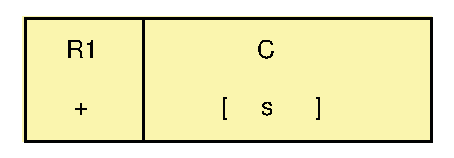
\includegraphics[width=0.23\textwidth]{figs/AppendixB/Tags/Implied.pdf}} & \multirow{3}{12cm}{The ``+'' traceability status indicates that the behavior is not explicitly stated in the original requirements but is implied by the requirement. The color ``yellow'' is used for implied behavior.} \\*
 &&\\
 &&\\
 \hline
 \multirow{3}{*}{Missing} & \multirow{3}{*}{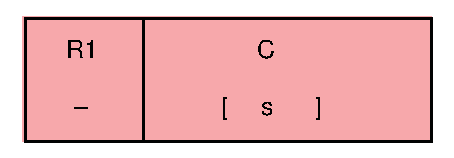
\includegraphics[width=0.23\textwidth]{figs/AppendixB/Tags/Missing.pdf}}  & \multirow{3}{12cm}{The ``-'' traceability status indicates that the behavior is missing from the original requirements and is needed for completeness. The color ``red'' is used for missing behavior.}\\*
 &&\\
 &&\\
 \hline
 \multirow{3}{*}{Design} & \multirow{3}{*}{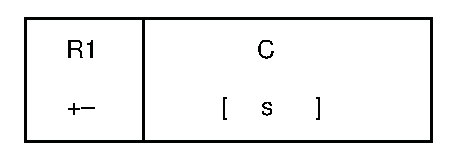
\includegraphics[width=0.23\textwidth]{figs/AppendixB/Tags/Updated.pdf}} & \multirow{3}{12cm}{The ``+-'' traceability status indicates that the behavior is a refinement of the original requirements, indicating that the behavior is implied but the detail to describe it is missing.} \\*
 &&\\
 &&\\
 \hline
 \multirow{6}{*}{Updated} & \multirow{6}{*}{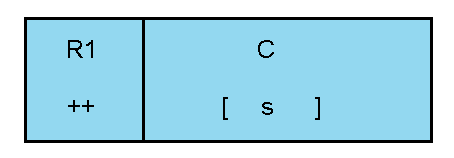
\includegraphics[width=0.23\textwidth]{figs/AppendixB/Tags/Refinement.pdf}}  & \multirow{6}{12cm}{The ``++' traceability status indicates that the behavior has been added in the post-development or maintainence phase. The color ``blue'' is used for updated behavior. Where there are different series of changes / upgrades we use ++v1.0, ++v2.0, etc to indicate the particular upgrade series.}\\*
 &&\\
 &&\\
 &&\\
 &&\\
 &&\\
 \hline
 \multirow{5}{*}{Deleted} &  \multirow{5}{*}{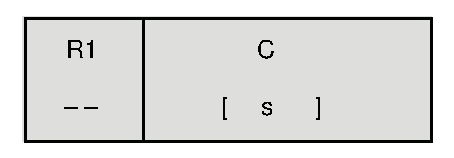
\includegraphics[width=0.23\textwidth]{figs/AppendixB/Tags/Deleted.pdf}} & \multirow{5}{12cm}{The ``--'' traceability status indicates that the behavior has been deleted from the behavior tree. The color ``grey'' is used for deleted behavior, but the nodes may also be hidden optionally by using tool support.} \\*
 &&\\
 &&\\
 &&\\
 &&\\
 \hline
\end{longtable}
\end{center}

\onehalfspacing

\subsection{Basic Nodes}

\singlespacing
\begin{center}
\begin{small}
\begin{tabular}[c]{|c|c|p{12cm}|}\hline
\textbf{Type} & \textbf{Graphical Notation} & \textbf{Description} \\ 
\hline
\hline
\multirow{3}{*}{State Realisation} & \multirow{3}{*}{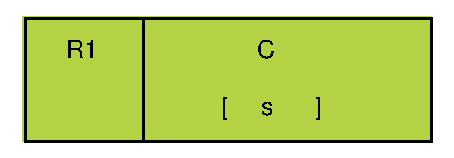
\includegraphics[width=0.23\textwidth]{figs/AppendixB/BasicNodes/StateRealisation.pdf}} & \multirow{3}{12cm}{Component C realises state s.} \\*
&&\\
&&\\
\hline
\multirow{3}{*}{System State Realisation} & \multirow{3}{*}{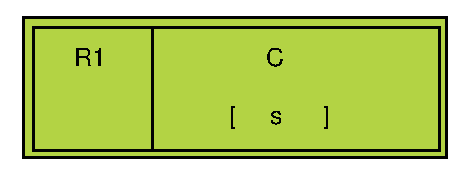
\includegraphics[width=0.23\textwidth]{figs/AppendixB/BasicNodes/SystemStateRealisation.pdf}}& \multirow{3}{12cm}{This is a state realisation decorated with a double box to indicate the component is a system component in the current context. There can only be one system component in each context.}\\*
&&\\*
&&\\*
\hline
\multirow{3}{*}{Selection} & \multirow{3}{*}{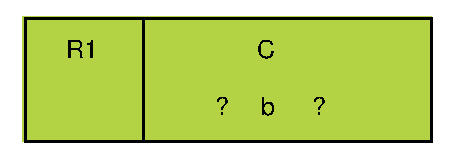
\includegraphics[width=0.23\textwidth]{figs/AppendixB/BasicNodes/Selection.pdf}} & \multirow{3}{12cm}{If condition $b$ evaluates to true, then pass control to child nodes otherwise terminate.}\\*
&&\\ 
&&\\
\hline
\multirow{3}{*}{Event} & \multirow{3}{*}{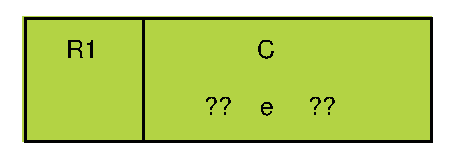
\includegraphics[width=0.23\textwidth]{figs/AppendixB/BasicNodes/Event.pdf}} & \multirow{3}{12cm}{Wait until event $e$ is received.} \\*
&&\\
&&\\
\hline
\multirow{3}{*}{Guard} & \multirow{3}{*}{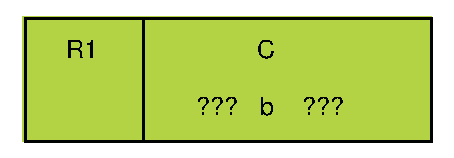
\includegraphics[width=0.23\textwidth]{figs/AppendixB/BasicNodes/Guard.pdf}} & \multirow{3}{12cm}{Wait until condition $b$ evaluates to true, then pass control to child nodes.} \\*
&&\\
&&\\
 \hline
\multirow{3}{*}{Internal Output} & \multirow{3}{*}{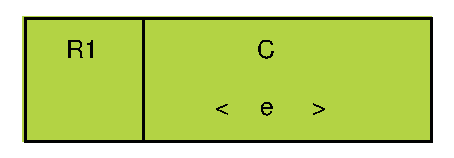
\includegraphics[width=0.23\textwidth]{figs/AppendixB/BasicNodes/IOEvent.pdf}}  & \multirow{3}{12cm}{Generate input $e$ and send to the system.} \\*
&&\\ 
&&\\
\hline
\multirow{3}{*}{Internal Input} & \multirow{3}{*}{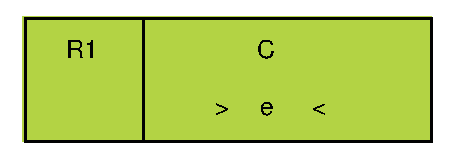
\includegraphics[width=0.23\textwidth]{figs/AppendixB/BasicNodes/IIEvent.pdf}} & \multirow{3}{12cm}{Wait for input $e$ from the system.} \\*
&&\\
&&\\
\hline
\multirow{3}{*}{External Output} & \multirow{3}{*}{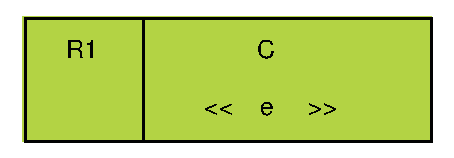
\includegraphics[width=0.23\textwidth]{figs/AppendixB/BasicNodes/EOEvent.pdf}} & \multirow{3}{12cm}{Generate output $e$ and send to the environment.} \\*
&&\\
&&\\
\hline
\multirow{3}{*}{External Input} & \multirow{3}{*}{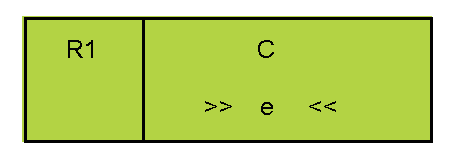
\includegraphics[width=0.23\textwidth]{figs/AppendixB/BasicNodes/EIEvent.pdf}} & \multirow{3}{12cm}{Wait for input $e$ to be received from the environment.} \\*
&&\\
&&\\
\hline
\multirow{3}{*}{Empty Node}& \multirow{3}{*}{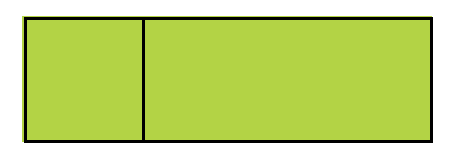
\includegraphics[width=0.23\textwidth]{figs/AppendixB/BasicNodes/Empty.pdf}} & \multirow{3}{12cm}{Empty Nodes can be used together with labels to be origins or destinations of node operators. Empty Nodes are also useful for grouping child nodes into multiple branch types.} \\*
&&\\
&&\\
\hline
\end{tabular}
\end{small}
\end{center}

\onehalfspacing

\subsection{Behavior Tree Composition}

\singlespacing
\begin{center}
\begin{longtable}[c]{|c|c|c|p{0.65\textwidth}|} \hline
\textbf{Type} & \textbf{Graphical Notation} &  \textbf{Description} \\*
\hline 
\hline
\multirow{6}{*}{Sequential Composition}&\multirow{6}{*}{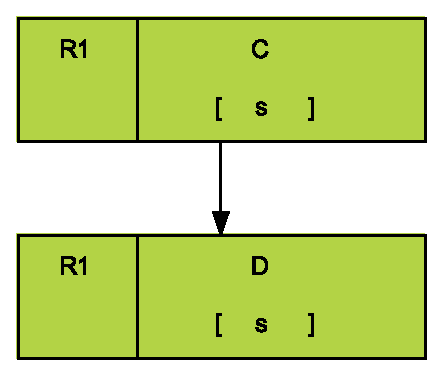
\includegraphics[width=0.189\textwidth]{figs/AppendixB/Composition/Sequential.pdf}} &\multirow{6}{0.65\textwidth}{Execute $N$, passing control to tree $T$. The behavior of concurrent BTs may be interleaved between $N$ and $T$.}\\*
&&\\*
&&\\*
&&\\*
&&\\*
&&\\*
%&&\\*
%&&\\
\hline
\multirow{4}{*}{Atomic Composition}&\multirow{4}{*}{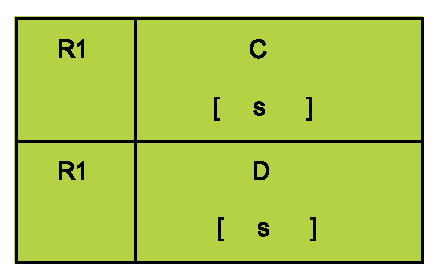
\includegraphics[width=0.189\textwidth]{figs/AppendixB/Composition/Atomic.pdf}} & \multirow{4}{0.65\textwidth}{Execute $N_1$ immediately followed by $N_2$, passing control to tree $T$. The behavior of concurrent BTs may not be interleaved between $N_1$ and $N_2$.} \\*
&&\\*
&&\\*
&&\\*
%``&&\\
\hline
\multirow{6}{*}{Parallel Branching}&\multirow{6}{*}{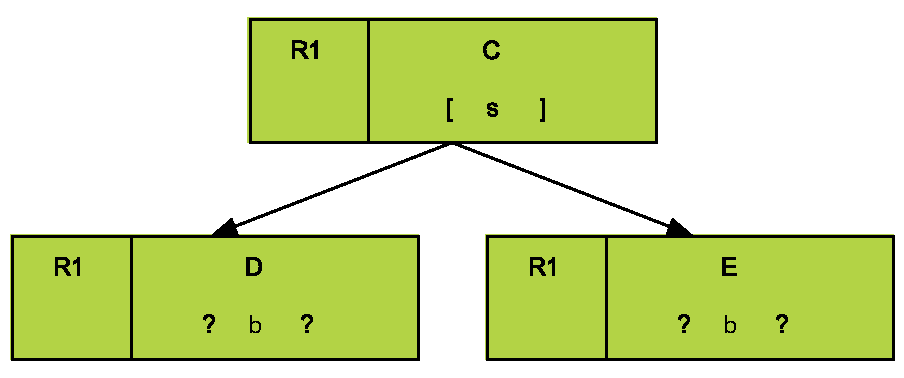
\includegraphics[width=0.4\textwidth]{figs/AppendixB/Composition/Parallel.pdf}} &  \multirow{6}{0.65\textwidth}{Execute $N$, passing control to both $T_1$ and $T_2$.} \\*
&&\\*
&&\\*
&&\\*
&&\\*
%&&\\*
%&&\\*
&&\\
\hline
\multirow{7}{*}{Alternative Branching}&\multirow{7}{*}{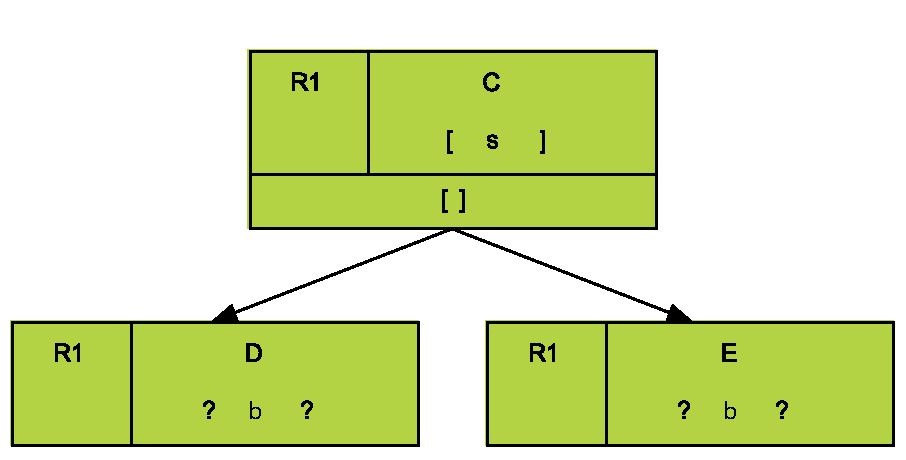
\includegraphics[width=0.4\textwidth]{figs/AppendixB/Composition/Alternative.pdf}}&  \multirow{7}{0.65\textwidth}{A nondeterministic choice is made between $T_1$ and $T_2$, depending on which is ready to execute (not blocked)} \\*
&&\\*
&&\\*
&&\\*
&&\\*
&&\\*
&&\\*
\hline
\end{longtable}
\end{center}

\subsection{Node Operators}

\begin{small}
\singlespacing
\begin{itemize}
\item Operators on source nodes match against the Component, Behavior, Behavior Type and Label (if present) of the destination node.
\item An operator may be prefixed by a label and a fullstop to refer to a destination node with a label e.g. $lbl.^{\wedge}$ indicates to revert to destination node with label $lbl$.
\end{itemize}
\end{small}

\singlespacing
\begin{center}
\begin{tabular}[c]{|c|c|p{12cm}|}\hline
\textbf{Type} & \textbf{Graphical Notation} & \textbf{Description} \\ 
\hline
\hline
\multirow{3}{*}{Reference} & \multirow{3}{*}{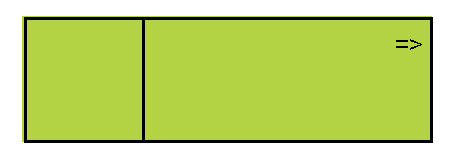
\includegraphics[width=0.23\textwidth]{figs/AppendixB/Operators/Reference.pdf}} & \multirow{3}{12cm}{Behave as the destination node. The destination node must appear in an alternative branch to the origin.} \\
&&\\
&&\\
\hline
 \multirow{3}{*}{Reversion} & \multirow{3}{*}{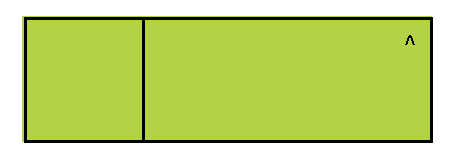
\includegraphics[width=0.23\textwidth]{figs/AppendixB/Operators/Reversion.pdf}} & \multirow{3}{12cm}{Behave as the destination node. The destination node must be an ancestor. All sibling behaviour is terminated.} \\
&&\\
&&\\
 \hline
 \multirow{3}{*}{Branch Kill} & \multirow{3}{*}{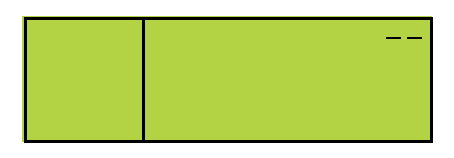
\includegraphics[width=0.23\textwidth]{figs/AppendixB/Operators/BranchKill.pdf}} & \multirow{3}{12cm}{Terminate all behavior associated with destination tree.}\\
&&\\
&&\\
 \hline
 \multirow{3}{*}{Synchronisation} & \multirow{3}{*}{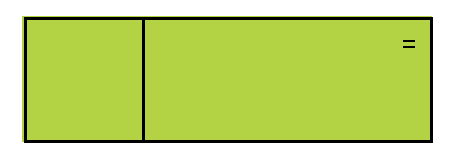
\includegraphics[width=0.23\textwidth]{figs/AppendixB/Operators/Synchronisation.pdf}} & \multirow{3}{12cm}{Wait for destination node (or nodes).}\\
&&\\
&&\\
 \hline
 \multirow{3}{*}{May} & \multirow{3}{*}{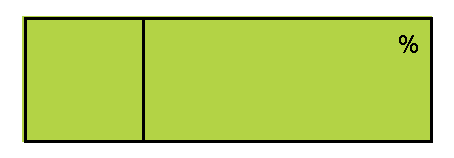
\includegraphics[width=0.23\textwidth]{figs/AppendixB/Operators/May.pdf}} & \multirow{3}{12cm}{The node may execute normally, or may have no effect.}\\
 &&\\
&&\\ 
 \hline
 \multirow{3}{*}{Conjunction} & \multirow{3}{*}{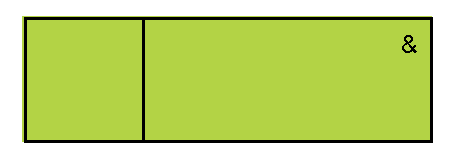
\includegraphics[width=0.23\textwidth]{figs/AppendixB/Operators/Conjunction.pdf}} & \multirow{9}{12cm}{The operators \&, $|$ and $XOR$ correspond to logical conjunction, disjunction and exclusive or respectively.}\\
 &&\\
&&\\
 \cline{1-2}
 \multirow{3}{*}{Disjunction} & \multirow{3}{*}{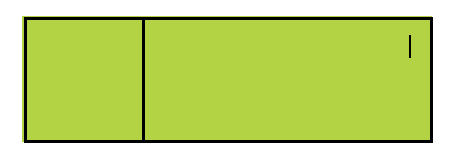
\includegraphics[width=0.23\textwidth]{figs/AppendixB/Operators/Disjunction.pdf}} & \\
 &&\\
&&\\
 \cline{1-2}
 \multirow{3}{*}{Exclusive OR} & \multirow{3}{*}{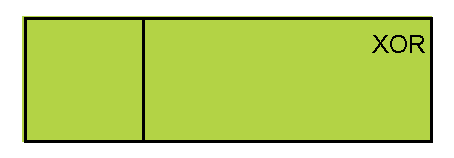
\includegraphics[width=0.23\textwidth]{figs/AppendixB/Operators/XOR.pdf}} & \\
 &&\\
&&\\
 \hline
\end{tabular}
\end{center}
\onehalfspacing

\clearpage


\end{landscape}
\end{document}